\documentclass[12pt, titlepage]{article}
\usepackage[shortlabels]{enumitem}
\usepackage{comment}
\usepackage{booktabs}
\usepackage{tabularx}
\usepackage{hyperref}
\usepackage{float}
\usepackage{soul}
\usepackage{changepage}
\usepackage{graphicx}
\usepackage{pdflscape}
\hypersetup{
    colorlinks,
    citecolor=blue,
    filecolor=black,
    linkcolor=red,
    urlcolor=blue
}
\usepackage[round]{natbib}
\usepackage[dvipsnames]{xcolor}

%% Comments

\usepackage{color}

\newif\ifcomments\commentstrue %displays comments
%\newif\ifcomments\commentsfalse %so that comments do not display

\ifcomments
\newcommand{\authornote}[3]{\textcolor{#1}{[#3 ---#2]}}
\newcommand{\todo}[1]{\textcolor{red}{[TODO: #1]}}
\else
\newcommand{\authornote}[3]{}
\newcommand{\todo}[1]{}
\fi

\newcommand{\wss}[1]{\authornote{blue}{SS}{#1}} 
\newcommand{\plt}[1]{\authornote{magenta}{TPLT}{#1}} %For explanation of the template
\newcommand{\an}[1]{\authornote{cyan}{Author}{#1}}

%% Common Parts

\newcommand{\progname}{ProgName} % PUT YOUR PROGRAM NAME HERE
\newcommand{\authname}{Team \#, Team Name
\\ Student 1 name
\\ Student 2 name
\\ Student 3 name
\\ Student 4 name} % AUTHOR NAMES                  

\usepackage{hyperref}
    \hypersetup{colorlinks=true, linkcolor=blue, citecolor=blue, filecolor=blue,
                urlcolor=blue, unicode=false}
    \urlstyle{same}
                                


\begin{document}

\title{System Verification and Validation Plan for \progname{}} 
\author{\authname}
\date{\today}
	
\maketitle

\pagenumbering{roman}

\begin{table}[H]
  \caption{\bf Revision History}
  \begin{tabularx}{\textwidth}{p{2.5cm}p{2.5cm}X}
  \toprule {\bf Date} & {\bf Developer} & {\bf Notes/Changes}\\
  \midrule
  Oct 31, 2022 & Timothy Chen & Added to 5.2, 5.3, 7.2\\
  Oct 31, 2022 & Edwin Do & Added section 4 for V\&V Plan\\
  Nov 1, 2022 & Abdul Nour Seddiki & Added to 5.1, 5.3\\
  Nov 2, 2022 & Joseph Braun & Added Section 3\\
  Nov 2, 2022 & Edwin Do & Added more content to section 4 \\
  Mar 4, 2023 & Edwin Do & Revised tests for non functional requirements\\
  Mar 4, 2023 & Timothy Chen & Revised Usability and Performance NFR test\\
  Mar 6, 2023 & Abdul Nour Seddiki & Revised tests for Functional Requirements \& fixed formatting\\
  Mar 8, 2023 & Edwin Do, Timothy Chen & Further revision of tests for non functional requirements\\
  Mar 8, 2023 & Edwin Do & Added unit tests for calculation and validation\\
  Mar 8, 2023 & Tyler Magarelli & Updated user experience survey for section 6.2\\
  Mar 8, 2023 & Timothy Chen & Added Unit Test Plan for Input Communication, Remote Access, Current State\\
  Apr 3, 2023 & Edwin Do & Updated Plan for SRS, Design, Implementation and Software\\
  Apr 3, 2023 & Timothy Chen & Updated user survey used\\
  Apr 3, 2023 & Edwin Do & Updated relevant documentation\\
  Apr 3, 2023 & Timothy Chen & Updated Non-functional requirements\\
  Apr 3, 2023 & Tyler Magarelli & Updated Traceability Matrix\\
  Apr 3, 2023 & Abdul Nour Seddiki & Updated System tests for Functional Requirements\\
  \bottomrule
  \end{tabularx}
  \end{table}
  

\newpage

\tableofcontents

\listoftables
%\wss{Remove this section if it isn't needed}

%\listoffigures
%\wss{Remove this section if it isn't needed}

\newpage

\section{Symbols, Abbreviations and Acronyms}

\renewcommand{\arraystretch}{1.2}
\begin{tabular}{l l} 
  \toprule		
  \textbf{symbol} & \textbf{description}\\
  \midrule 
  T & Test\\
  SRS & Software Requirements Specifications \\
  MG & Module Guide\\
  MIS & Module Interface Specification\\
  VS & Visual Studio\\
  UWP & Universal Windows Platform\\
  INTERACT\_TIME & Maximum time taken for user to interact with application \\
  MAX\_MISTAKE & Maximum mistakes allowed  \\
  MAX\_SIZE & Maximum size of the application \\ 
  MIN\_UPTIME & Minimum time required for application to stay alive  \\ 
  MIN\_SAMPLE\_RATE & Minimum sampling rate required\\
  TIME\_ACCEPTED & Maximum time for updates to occur \\
  ACCEPTED\_SIGFIG & Number of significant digits \\
  \bottomrule
\end{tabular}\\

\newpage

\pagenumbering{arabic}

\section{General Information}

\subsection{Summary}

The purpose of this document is to provide a detailed plan for the testing of our system. This will include:
\begin{itemize}
  \item Verification and Validation Plan
  \item System Test Description
  \item Unit Test Description
\end{itemize}

\subsection{Objectives}

The objectives of testing are to ensure that all functional and non-functional requirements of the system are being met. It is important to include both unit tests as well as system tests, as issues may arise when components are connected together in the system. 

\subsection{Relevant Documentation}

Relevant documentation includes:
\begin{itemize}
  \item \href{../SRS/SRS.pdf}{SRS} : This document contains information regarding the functional and non-functional requirements of the application which will be referenced to ensure that the testing of the application shows confidence that each requirement has been met.
  \item \href{../Design/SoftDetailedDes/MIS.pdf}{MIS} : This document contains information regarding the interface of each software module and the interaction between them. This will be referenced to ensure that the design and implementation of the application follow this document and that any design/logical flaws are identified, and it will be updated swiftly.
\end{itemize}

\section{Plan}
% RUBRIC
% 'Team member's roles for testing are clear;  
% This may involve switching roles between verification tasks 
% (say between SRS verification, hardware verification, and code verification).  
% Clear, specific and feasible plan for SRS verification; 
% Clear specific and feasible plan for Design verification; 
% Clear specific and feasible plan for implementation verification.  
% Automated testing and verification tools are specific.  
% Software validation plan is clear, specific and feasible.

% \wss{Introduce this section.   You can provide a roadmap of the sections to
%   come.}

  This section of planning will outline our approaches to cover the requirements outlined in various areas such as the \href{../SRS/SRS.pdf}{SRS} document, \href{../HazardAnalysis/HazardAnalysis.pdf}{Hazard Analysis document}, our implementation, and design. In addition, the responsibilities of each team member will be outlined as a reference. The responsibilities may change as needed when a team member finishes early or if another team member encounters an issue. 
  Tools that will be used for automated unit testing and linting will also be introduced.\\

  The following topics will be covered:

  \begin{itemize}
    \item The verification and validation team along with their respective responsibilities
    \item Our approach and plan toward the SRS Verification plan
    \item Our approach and plan toward the Design Verification plan
    \item Our approach and plan toward the Implementation verification plan
    \item Any testing and verification tools we plan to use
  \end{itemize}


\subsection{Verification and Validation Team}

% \wss{You, your classmates and the course instructor.  Maybe your supervisor.
%   You shoud do more than list names.  You should say what each person's role is
%   for the project.  A table is a good way to summarize this information.}

  Below is a table outlining the members of the Verification and Validation team along with their respective responsibilities.
  Note that the listed responsibilities are only used as a guideline, responsibilities can shift between team members on an as-per-needed basis (i.e. if another team member is stuck or needs help, other team members may join in and help resolve the issue).

  \begin{table}[H]
    \centering
    \caption{Team and Responsibilities}
    \label{my-label}
    \begin{tabular}{|c|c|c|}
      \hline
      \textbf{Team Member} & \textbf{Role Name} & \textbf{Responsibilities}   \\ \hline
      Edwin Do & 
      \begin{tabular}{@{}c@{}}Software and SRS Tester\end{tabular} & 
      \begin{tabular}{@{}c@{}}Ensures that all requirements are valid \\ 
        and verified under the scope of software \\
        capabilities in this project and the SRS\end{tabular} \\ \hline
      
      Timothy Chen & 
      \begin{tabular}{@{}c@{}}Software Tester\end{tabular} & 
      \begin{tabular}{@{}c@{}}Ensures that all requirements are met \\ 
        and verified under the scope of software \\
        capabilities in this project\end{tabular} \\ \hline
      
      Tyler Magarelli & 
      \begin{tabular}{@{}c@{}}Software Tester\end{tabular} & 
      \begin{tabular}{@{}c@{}}Ensures that all requirements are met\\ 
        and verified under the scope of software \\
        capabilities in this project\end{tabular} \\ \hline
      
      Joseph Braun & 
      \begin{tabular}{@{}c@{}}Hardware Tester\end{tabular} & 
      \begin{tabular}{@{}c@{}}Ensures that all requirements are met \\ 
        and verified under the scope of hardware \\
        capabilities in this project\end{tabular} \\ \hline
      
      Abdul Nour Seddiki & 
      \begin{tabular}{@{}c@{}}Hardware Tester\end{tabular} & 
      \begin{tabular}{@{}c@{}}Ensures that all requirements are met \\ 
        and verified under the scope of hardware \\
        capabilities in this project\end{tabular} \\ \hline

      Dr. Hatem Zurob & 
      \begin{tabular}{@{}c@{}}Supervisor\end{tabular} & 
      \begin{tabular}{@{}c@{}}Ensures that all requirements are valid \\ 
        and meets the expected result\end{tabular} \\ \hline
    \end{tabular}
  \end{table}

\subsection{SRS Verification Plan}

% \wss{List any approaches you intend to use for SRS verification.  This may just
%   be ad hoc feedback from reviewers, like your classmates, or you may have
%   something more rigorous/systematic in mind..}

% \wss{Remember you have an SRS checklist}

\noindent As part of the SRS verification process, our team intends on revisiting the \href{../SRS/SRS.pdf}{SRS document} on a bi-weekly basis to verify that 
the requirements are up to date and in sync with the project goal. 
The team will do so by going over each of the functional and non-functional requirements collectively. When reviewing a specific requirement, the team will discuss on the updated progress and/or relevance to the project. When a requirement is no longer valid or relevant to the project, the team will then decide on whether the requirement requires modification or removal from the SRS. This enables the team to be able to use the SRS document as a "source of truth" throughout the development of the project. This will also allow us to uncover any newly discover risks or hazards as requirements are modified which can be reflected in the \href{../HazardAnalysis/HazardAnalysis.pdf}{Hazard Analysis document}. \\

\noindent Any new changes within the two-week window will be noted and discussed at the bi-weekly meeting. At each bi-weekly review, the team also plans on using the SRS checklist as a guideline throughout
the meeting to ensure all components are met.\\

\noindent  In addition, the team will use ad-hoc feedback from reviewers such as classmates from our 4G06 Capstone class, instructor, supervisor, and teaching assistants. Feedback from classmates can be found on GitHub as GitHub Issues. The team will review any new issues during the bi-weekly meeting and discuss each issue collectively. Feedback from the teaching assistants can be found on Avenue, where the team will also review the feedback and discuss the modifications necessary to the document. This will act as a supplementary addition if any element of the SRS 
is out of date, missing, or requires additional changes.

\subsection{Design Verification Plan}

As part of the design verification process, the team will review the design outlined in the \href{../Design/SoftDetailedDes/MIS.pdf}{MIS document} on a bi-weekly basis. As development progresses, the design may be modified and changed throughout. The team will reflect those modifications in the MIS document. In addition, as the team reviews the MIS document, it will allow the team to identify any gaps or redundancy in the design as well as new risks and hazards, which can trigger additional changes to the implementation. Similar to the SRS, the team will use the MIS as a "source of truth" to ensure that all team members are aware of the current design and logic of the implementation. \\

\noindent The team will also use the MIS checklist at each of our bi-weekly meetings ensuring that all components are met correctly as modifications are made. Feedback from our classmates can also be received through GitHub as GitHub Issues and will be reviewed and discussed by the team during each meeting. As part of the review for each issue, the team will identify the issue, discuss potential fixes, and select and apply the agreed-upon modification. This will allow every member to be aware of each modification as well as the rationale behind it. By doing so, logical flaws are spotted more likely since every member is aware of all previous contexts and changes. 

\noindent  In addition, the team will use feedback from reviewers such as classmates from our 4G06 Capstone class as well
as instructor, supervisor, and teaching assistants. This will help further assist our team to ensure that the design is free from 
any logical flaws and is able to help meet the outlined requirements. 

% \wss{Plans for design verification}

% \wss{The review will include reviews by your classmates}

% \wss{Remember you have MG and MIS checklists}

\subsection{Implementation Verification Plan}

% [Point to other tests and unit testing plan]

Throughout the development phase of this project, the team will use GitHub Issues to identify features to be implemented. Team members will choose a feature to implement, and once completed will create a pull request linked to the issue. Each pull request will require at least two other team members to inspect and review the code ensuring that it meets the requirement and design discussed. A pipeline can also be implemented in GitHub to ensure that the build in the main branch is always stable. \\

\noindent Testing will be conducted by the team throughout the implementation process to ensure functional requirements are met (refer to \hyperref[FR-T]{Tests for Functional Requirements}).\\

\noindent Non-functional requirements will be tested during a user demo, where the user will attempt to run and control an experiment with no prior experience with the application. A user survey will be conducted after the demo to determine if the application has met specific non-functional requirements (refer to \hyperref[SQ]{Survey Questions}). After administering the survey, we will use the results as well as any additional feedback from the user to improve on the application. Some non-functional requirements tests will be conducted by the team rather than the user (refer to \hyperref[NF-T]{Tests for Non-Functional Requirements}).\\

\noindent Unit tests will be performed by the team. Each module as described in the MG will be implemented by one or two team members. After a module is completed, unit testing will be performed on that module (Refer to \hyperref[UTD]{Unit Test Description}).\\

 

% \wss{You should at least point to the tests listed in this document and the unit
%   testing plan.}

% \wss{In this section you would also give any details of any plans for static verification of
%   the implementation.  Potential techniques include code walkthroughs, code
%   inspection, static analyzers, etc.}

\subsection{Automated Testing and Verification Tools}

The application will be a Windows Presentation Foundation (WPF) application built using Microsoft Visual Studio (VS) in C\# and XAML. \\

\noindent Majority of the project's testing will be conducted within VS. 
For unit testing, the team will use the built-in features of Unit Test Applications in VS to create unit tests projects and unit tests.\\

\noindent Code coverage tests are also covered within the suite of tools available within VS. The team will be able to create testing suites and 
unit tests for the VS project. The team also plans on using the results of the code coverage
tests to identify which portion of the project's code is not covered by our tests. Uncovered blocks of code can be colour-coded to signify to 
the developer that no current test covers that block of code. Other metrics such as the number of lines covered and the \% of a block covered will be 
summarized per code coverage project to help indicate where more testing efforts are needed. \\

\noindent Using Visual Studio's IDE extensions, the team plans on using SonarLint and CSharpier as its linter and formatting tool for C\# respectively. 

% \wss{What tools are you using for automated testing.  Likely a unit testing
%   framework and maybe a profiling tool, like ValGrind.  Other possible tools
%   include a static analyzer, make, continuous integration tools, test coverage
%   tools, etc.  Explain your plans for summarizing code coverage metrics.
%   Linters are another important class of tools.  For the programming language
%   you select, you should look at the available linters.  There may also be tools
%   that verify that coding standards have been respected, like flake9 for
%   Python.}

% \wss{The details of this section will likely evolve as you get closer to the
%   implementation.}

\subsection{Software Validation Plan}

As part of our Software Validation process, the team intends to utilize the sample data that is provided by Dr. Zurob. The sample data will provide the team with expected results that can be used to evaluate the accuracy of the application. The expected results must accurate to at least ACCEPTED\_SIGFIG in order for the team to accept the results. Otherwise, the team will conclude that the software is not yet valid. The primary concerns for the results are the values of resistivity and voltage. This will allow the team to know if the calculations of the resistivity are correct and if the application is able to receive accurate measurements of voltage. If either of these components is incorrect, then the application will be invalid. 

% Specific margin of error 

% Use sample data provided by Dr.Zurob to ensure the accuracy of data 

% \wss{If there is any external data that can be used for validation, you should
%   point to it here.  If there are no plans for validation, you should state that
%   here.}

\section{System Test Description}
	
\subsection{Tests for Functional Requirements}
\label{FR-T}
\begin{enumerate}[{FR-T}1.]
    \item\label{T1} - Control: Dynamic \& Manual\\ 
    - Relevant Functional Requirements: FR1\\
    - Initial State: Entire system is set up and the application is running.\\
    - Input: Developers will initialize the current source with supply parameters and initialize the nanovoltmeter.\\
    - Output: The application shall input the parameters of the current supply and set them to the current source appropriately, then enable and disable the current. The current level shall be displayed appropriately. The nanovoltmeter shall be reset and on hold awaiting capture initialization.\\
    - Test Case Derivation: This test ensures that the input parameters are properly and promptly received by the instruments.\\
    - How the test will be performed: The test will be performed by developers. By specifying current source parameters and then clicking the “Set All”, "ON", and "OFF" buttons. While simultaneously monitoring both the values displayed on the current source and the ones displayed in the application, as well as making sure that the current supply is being toggled using the appropriate buttons and indicated clearly.
    
    \item\label{T2} - Control: Dynamic \& Manual\\ 
    - Relevant Functional Requirements: FR1\\
    - Initial State: Entire system is set up and the application is running.\\
    - Input: Developers will initialize the current source with supply parameters, initialize the nanovoltmeter and capture measurements, set up a sample, and demonstrate the main function of the application.\\
    - Output: The application shall input the parameters of the current supply and set them to the current source appropriately, then enable and disable the current. The current level shall be displayed appropriately. The nanovoltmeter shall be reset and the application shall display the voltage levels and other values appropriately when capture is started.\\
    - Test Case Derivation: This test ensures that the output measurements are properly displayed on the user interface in real-time.\\
    - How the test will be performed: The test will be performed by developers. By clicking the “Start Capture” button. Simultaneously monitoring both the values displayed on the nanovoltmeter and the ones displayed in the application while observing for latency.
    
    \item\label{T3} - Control: Dynamic \& Manual\\
    - Relevant Functional Requirements: FR1\\
    - Initial State: Entire system is set up and the application is running.\\
    - Input: Developers will initialize the current source with supply parameters, initialize the nanovoltmeter and capture measurements, set up a sample, and demonstrate the main function of the application.\\
    - Output: The current source shall be reset and the application shall input the parameters of the current supply and set them to the current source appropriately, then enabling and disabling the current. The current level shall be displayed appropriately. The nanovoltmeter shall be reset and the application shall display the voltage levels appropriately when capture is started. The application shall calculate and display the resistivity of the metallic sample based on values obtained from the measurement devices.\\
    - Test Case Derivation: This test ensures that the background calculation results are properly displayed on the user interface in real-time.\\
    - How the test will be performed: The test will be performed by developers. By clicking the “Start Capture” button. Then verifying the resistivity calculations by taking samples from the logs and doing a manual calculation. Simultaneously monitoring both the values displayed on the devices and the ones displayed in the application while observing for latency.

    \item\label{T4} - Control: Dynamic \& Manual\\
    - Relevant Functional Requirements: FR1, FR2\\
    - Initial State: Entire system is set up and the application is running.\\
    - Input: Developers will control the "Acquisition Rate" of the voltage measurement.\\
    - Output: The nanovoltmeter shall indicate a change in the internal sampling rate. The front display shall work at a rate faster or slower than the default rate.\\
    - Test Case Derivation: This test ensures that the acquisition rate is able to be relayed to the nanovoltmeter by the application promptly.\\
    - How the test will be performed: The test will be performed by developers. By changing the value in the "Acquisition Rate" textbox and clicking "Set". Simultaneously monitoring the rate of display on the nanovoltmeter before and after the rate changes are set.
    
    \item\label{T5} - Control: Dynamic \& Manual\\ 
    - Relevant Functional Requirements: FR1, FR2\\
    - Initial State: Entire system is set up and the application is running.\\
    - Input: Developers will control the "Acquisition Rate" of the voltage measurement.\\
    - Output: The nanovoltmeter shall indicate a change in the internal sampling rate. The front display shall work at a rate faster or slower than the default rate, and the application shall follow suit when displaying measurements and calculations.\\
    - Test Case Derivation: This test ensures that changing the acquisition rate changes the speed at which measurements and calculations are displayed on the user interface.\\
    - How the test will be performed: The test will be performed by developers. By changing the value in the "Acquisition Rate" textbox and clicking "Set". Simultaneously monitoring the rate of measurements and calculations displayed on the app before and after the rate changes are set.

    \item\label{T6} - Control: Dynamic \& Manual\\ 
    - Relevant Functional Requirements: FR3\\
    - Initial State: Entire system is set up and both the application and the remote web client are running.\\
    - Input: Developers will prompt a wireless connection to the control computer and check for current status.\\
    - Output: The application is able to be monitored using the web client.\\
    - Test Case Derivation: This test ensures that the remote client is able to be updated on the status of an experiment.\\
    - How the test will be performed: The test will be performed by developers communicating remotely with the control computer through a web client. The main application's status is known. Remotely, the testing developer will click the “Refresh” button on the web client and that will prompt the main app to update its current status to the web client.

    \item\label{T7} - Control: Dynamic \& Manual\\ 
    - Relevant Functional Requirements: FR1, FR3\\
    - Initial State: Entire system is set up and both the application and the remote web client are running.\\
    - Input: Developers will prompt a wireless connection to the control computer and start and stop an experiment.\\
    - Output: The application is able to be controlled using the web client; the capture is started and stopped remotely.\\
    - Test Case Derivation: This test ensures that the remote client is able to start and stop experiments.\\
    - How the test will be performed: The test will be performed by developers communicating remotely with the control computer through a web client. Remotely, the testing developer will click the “Start/Stop Experiment” button on the web client and that will prompt the main app to start and stop capture as well as display a notification of the updates.

    \item\label{T8} - Control: Dynamic \& Manual\\ 
    - Relevant Functional Requirements: FR1, FR3\\
    - Initial State: Entire system is set up and both the application and the remote web client are running.\\
    - Input: Developers will prompt a wireless connection to the control computer and turn the current output on and off.\\
    - Output: The application is able to be controlled using the web client; the current output is toggled remotely.\\
    - Test Case Derivation: This test ensures that the remote client is able to toggle the current supply output.\\
    - How the test will be performed: The test will be performed by developers communicating remotely with the control computer through a web client. Remotely, the testing developer will click the “Turn Current Supply ON/OFF” button on the web client and that will prompt the main app to toggle the current supply as well as display a notification of the updates.

    \item\label{T9} - Control: Dynamic \& Manual\\ 
    - Relevant Functional Requirements: FR1, FR4\\
    - Initial State: Entire system is set up, connected to a sample, and the application is running.\\
    - Input: Developers will start an experiment.\\
    - Output: The application displays a graph that shows real-time values and calculations.\\
    - Test Case Derivation: This test ensures that the user interface displays the measurements and calculations in graphical output.\\
    - How the test will be performed: The test will be performed by developers. Initializing the current source and voltmeter, then turning the current supply on and starting data capture. Then observing the graph in the application window.

    \item\label{T10} - Control: Dynamic \& Manual\\ 
    - Relevant Functional Requirements: FR1, FR4\\
    - Initial State: Entire system is set up, connected to a sample, and the application is running.\\
    - Input: Developers will start an experiment and adjust the graph.\\
    - Output: The application displays real-time values and calculations in an adjustable graph.\\
    - Test Case Derivation: This test ensures that the graphical output is adjustable.\\
    - How the test will be performed: The test will be performed by developers. Initializing the current source and voltmeter, then turning the current supply on and starting data capture. Then observing, zooming, navigating, and changing display parameters/axes of the graph in the application window.

    \item\label{T11} - Control: Dynamic \& Manual\\ 
    - Relevant Functional Requirements: FR5\\
    - Initial State: Entire system is set up, connected to a sample, the application is running, and an experiment is ongoing.\\
    - Input: Developers will stop the running experiment.\\
    - Output: The application shall save a ".CSV" file on the control computer.\\
    - Test Case Derivation: This test ensures that the application generates a ".CSV" file.\\
    - How the test will be performed: The test will be performed by developers. When enough data has been captured, they shall stop the experiment and check the documents folder in the control computer for the generated ".CSV" file.

    \item\label{T12} - Control: Dynamic \& Manual\\ 
    - Relevant Functional Requirements: FR1, FR5\\
    - Initial State: Entire system is set up, connected to a sample, the application is running, and an experiment is ongoing.\\
    - Input: Developers will stop the running experiment.\\
    - Output: The saved ".CSV" file on the control computer shall contain the measurements and calculations of the experiment.\\
    - Test Case Derivation: This test ensures that the generated ".CSV" file contains measurement and calculation data.\\
    - How the test will be performed: The test will be performed by developers. When enough data has been captured, they shall stop the experiment and open the generated file, checking for measurements and calculations being stored appropriately.

    \item\label{T13} - Control: Dynamic \& Manual\\ 
    - Relevant Functional Requirements: FR6\\
    - Initial State: The installation package exists as a compressed "ZIP" folder.\\
    - Input: Developers will uncompress the "ZIP" folder and check for a ".exe" executable file.\\
    - Output: The "ZIP" folder contains a ".exe" executable file.\\
    - Test Case Derivation: This test ensures that the installation package includes an executable file.\\
    - How the test will be performed: The test will be performed by developers. They will right-click the acquired "ZIP" folder, extract all contents into the desired source folder for the main application, and look for a ".exe" executable file.

    \item\label{T13} - Control: Dynamic \& Manual\\ 
    - Relevant Functional Requirements: FR6\\
    - Initial State: The installation package folder is uncompressed and an executable file exists. The operating system in use is Microsoft Windows.\\
    - Input: Developers will attempt to launch the ".exe" executable file.\\
    - Output: The ".exe" executable file successfully launches the application.\\
    - Test Case Derivation: This test ensures that the executable file works on the Microsoft Windows operating system and that the application can be directly run through it.\\
    - How the test will be performed: The test will be performed by developers. They will right-click the ".exe" executable file found in the source folder, choose "Open", and observe the application window being launched.


\end{enumerate}

\subsection{Tests for Nonfunctional Requirements}
\label{NF-T}
\subsubsection{Appearance Test}

\begin{adjustwidth}{2.2em}{0pt}
\begin{enumerate}[{NF-AT}1.]
    
    \item Type: Static \& Manual \\ \label{AT1}
    Initial State: Application is opened and ready for use.\\
    Input/Condition: The user will follow a simple set of instructions to explore the application, followed by a survey.\\
    Output/Result: The survey result will indicate that the user agrees or disagrees that the application is uncomplicated. \\
    How the test will be performed: The test will be performed by the user. They will receive a survey with a question. If the user indicates they agree or strongly agree, then it will be considered successful. (Refer to \hyperref[SQ]{Survey Questions})
    
    \item Type: Static \& Manual\\ \label{AT2}
    Initial State: Application is opened and ready for use.\\
    Input/Condition: Developers will navigate the application by exploring every screen and state.\\
    Output/Result: If all sections of the applications is in English, then this test is considered a pass. Otherwise, it is considered a failure.\\
    How the test will be performed: Different sets of instructions are used to cover a subset of the application screens and states, each set of instructions is to be carried out by a developer to verify the result. 
  \end{enumerate}
\end{adjustwidth}

\subsubsection{Usability Test}

\begin{adjustwidth}{2.2em}{0pt}
\begin{enumerate}[{NF-UT}1.]
  \item Type: Dynamic \& Manual\\ \label{UT1}
  Initial State: Application is opened and ready for use.\\
  Input/Condition: The user has no prior experience with the product.\\
  Output/Result: The user with no prior experience can successfully complete each task without additional assistance.\\
  How the test will be performed: The user will be observed while completing the task. The test will pass if the user completes the task without additional assistance.

  \item Type: Dynamic \& Manual\\ \label{UT2}
  Initial State: Application is opened and ready for use.\\
  Input/Condition: The user will be asked to modify the voltage and current parameters of the application to match a sample experiment we provide.\\
  Output/Result: The user takes no more than \textsl{INTERACT\_TIME} to interact with the application and make the modifications to the voltage and current parameters matching the sample experiment provided.\\
  How the test will be performed: The users will be observed while completing the task. The test will pass if the user takes no more than \textsl{INTERACT\_TIME}.

  \item Type: Dynamic \& Manual \\ \label{UT3}
  Initial State: Application is opened and ready for use.\\
  Input/Condition: The user will use the application by following a predefined set of tasks.\\
  Output/Result: The total number of mistakes made by the user when completing the tasks by interacting with the application should be no more than \textsl{MAX\_MISTAKE}.\\
  How the test will be performed: The observer will record the number of mistakes that they observe as the user completes the set of tasks.

  \item Type: Dynamic \& Manual\\ \label{UT4}
  Initial State: The application will be closed.\\
  Input/Condition: The user will open the application and perform a set of tasks listed for a sample experiment. Users then will be asked to return the next day to perform the same set of tasks.\\
  Output/Result:  The time that the user takes to complete the set of tasks for the second time will be less than the time taken for the first time.\\
  How the test will be performed: The user will be observed and timed while completing the set of tasks both times. The test will pass if the user completes the set of tasks in the same or less amount of time the next day.

  \item Type: Static \& Manual\\ \label{UT5}
  Initial State: Application is opened and ready for use.\\
  Input/Condition: The user will input sample parameters and the application will perform calculations.\\
  Output/Result: The application will display the result of the application and the user will not know how the calculations are performed \\
  How the test will be performed: The user will be observed while performing the task and asked to fill out an usability survey question. If the user is unaware of how the calculations were performed, the test will pass.

  \item Type: Static \& Manual\\ \label{UT6}
  Initial State: The application will be installed on the research device.\\
  Input/Condition: The size of the application will be checked manually.\\
  Output/Result: Application capacity on the device will be no more than \textsl{MAX\_SIZE}. \\
  How the test will be performed: We will open the file properties of the application and verify that the size of the application is less than or equal to \textsl{MAX\_SIZE}.
\end{enumerate}
\end{adjustwidth}

\subsubsection{Performance Test}

\begin{adjustwidth}{2.2em}{0pt}
\begin{enumerate}[{NF-PT}1.]
  \item Type: Dynamic \& Manual \\ \label{PT1}
  Initial State: The application is installed and running with measurement devices connected to a sample.\\
  Input/Condition: Set \textsl{MIN\_SAMPLE\_RATE} and start thermal treatment of sample.\\
  Output/Result: The application's output sample rate should be greater or equal to \textsl{MIN\_SAMPLE\_RATE}.\\
  How the test will be performed: The application sample rate will be set in the interface. When the experiment has started, we will observe the sample rate and compare it with the sample rate set in the interface. The test will pass if the observed sample rate is greater or equal to \textsl{MIN\_SAMPLE\_RATE}.
  
  \item Type: Dynamic \& Manual\\ \label{PT2}
  Initial State: The application is installed and running.\\
  Input/Condition: The user will be given parameters to change.\\
  Output/Result: Application will reflect changes within \textsl{TIME\_ACCEPTED}.\\
  How the test will be performed: The user will make modifications and we will observe how long the application takes to reflect the changes. 

  \item Type: Dynamic \& Manual\\ \label{PT3}
  Initial State: The application is installed and running with measurement devices connected to a sample.\\
  Input/Condition: Thermal treatment sample data will be read into the device.\\
  Output/Result: The sample reading from the thermal treatment will be accurate to \textsl{ACCEPTED\_SIGFIG} number of significant digits.\\
  How the test will be performed: Thermal treatment sample will be started, values read in from the device will be observed and compared to previous data of the thermal treatment sample given by Dr. Zurob. The test will pass if the result is correct up to the number of {ACCEPTED\_SIGFIG} significant digits.

  \item Type: Dynamic \& Manual\\ \label{PT4}
  Initial State: The application is installed and running with measurement devices connected to a sample.\\
  Input/Condition: The application will be opened and the user will interact with it.\\
  Output/Result: The application will be up and running for at least \textsl{MIN\_UPTIME} and for the entire duration of the task given to the user to perform.\\
  How the test will be performed: The user will complete a set of tasks using the application and the application will be left running for at least \textsl{MIN\_UPTIME} afterward.

\end{enumerate}
\end{adjustwidth}

\subsubsection{Operational Test}

\begin{adjustwidth}{2.2em}{0pt}
\begin{enumerate}[{NF-OT}1.]
    \item Type: Static \& Manual\\ \label{OT1}
    Initial State: The application is opened and ready with a keyboard and mouse connected to the device.\\
    Input/Condition: The user will interact with the application with a mouse and keyboard.\\
    Output/Result: The application will accurately and correctly reflect the inputs from the mouse and keyboard provided by the user.\\
    How the test will be performed: The user will be asked to perform a simple set of instructions using the mouse and keyboard such as clicking and typing.
    
    \item Type: Static \& Manual\\ \label{OT2}
    Initial State: A machine/computer that does not have the application installed.\\
    Input/Condition: The user will be asked to install the application on the machine/computer with a user guide.\\
    Output/Result: User successfully installed the application on the machine/computer.\\
    How the test will be performed: The test will be performed by the user. Users will be given a user guide with instructions to follow for the installation of the application. The user will be asked to install the application.
\end{enumerate}
\end{adjustwidth}

\subsubsection{Maintainability/Support Test}

\begin{adjustwidth}{2.2em}{0pt}
\begin{enumerate}[{NF-MT}1.]
    \item Type: Static \& Manual\\ \label{MT1}
    Initial State: A machine/computer that does not have the application installed.\\
    Input/Condition: The application will be installed on the device and connected to the required measurement devices.\\
    Output/Result: The application is able to operate smoothly without error with the connected measuring devices.\\
    How the test will be performed: The test will be performed by a developer installing the application onto a lab computer running Windows 10.
\end{enumerate}
\end{adjustwidth}

\subsubsection{Security Test}

\begin{adjustwidth}{2.2em}{0pt}
\begin{enumerate}[{NF-ST}1.]
    \item Type: Static \& Manual\\ \label{ST1}
    Initial State: Application is opened and ready to use.\\
    Input/Condition: The user will attempt to modify current parameters from the remote application without an SSL certificate installed or a VPN connection to Mac-WiFi if they are not on McMaster University Campus.\\
    Output/Result: The application will not reflect any modifications from the remote application.\\
    How the test will be performed: The test will be performed by a user with a missing SSL certificate or no connection to Mac-WiFi through VPN. The user will be asked to turn on/off the current. The test will pass if the application current remains in the same state as before the user performed the test.
    
    \item Type: Static \& Manual\\ \label{ST2}
    Initial State: Application is opened and ready to use.\\
    Input/Condition: The user will be asked to start an experiment from the remote application with an SSL certificate installed and connected to Mac-WiFi through McMaster Campus or VPN.\\
    Output/Result: The changes are accepted and reflected in the application interface.\\
    How the test will be performed: The test will be performed by users who have an SSL certificate installed and connected to Mac-WiFi through McMaster Campus or VPN. The users will be asked to start the capture. The test will pass if the application starts capture after the user selects the option on the remote application.
\end{enumerate}
\end{adjustwidth}

\subsubsection{Cultural Test}

\begin{adjustwidth}{2.2em}{0pt}
\begin{enumerate}[{NF-CT}1.]
    \item Type: Static \& Manual\\ \label{CT1}
    Initial State: Application is opened and ready to use.\\
    Input/Condition: The user will explore the application through a demo/test account. \\
    Output/Result: The survey result will indicate that the user agrees or disagrees that the graphics and wording are not offensive or inappropriate.\\
    How the test will be performed: The test will be performed by the user. They will receive a survey with a question. If the user indicates that they agree or strongly agree that graphics and wording are not offensive or inappropriate, then it will be considered successful. (Refer to \hyperref[SQ]{Survey Questions})
\end{enumerate}
\end{adjustwidth}

\subsubsection{Health and Safety Test}

\begin{adjustwidth}{2.2em}{0pt}
\begin{enumerate}[{NF-HT}1.] 
    \item Type: Static \& Manual\\ \label{HT1}
    Initial State: Application is opened and ready to use.\\
    Input/Condition: The user will explore the application through a demo/test account. \\
    Output/Result: The survey result will indicate that the user agrees or disagrees that the application does not cause/pose any health concerns.\\
    How the test will be performed: The test will be performed by the user. They will receive a survey with a question. If the user indicates that they agree or strongly agree that the application is free from health and safety concerns, then it will be considered successful. (Refer to \hyperref[SQ]{Survey Questions}).  
\end{enumerate}
\end{adjustwidth}

\newpage
\subsection{Traceability Between Test Cases and Requirements}

\begin{table}[h!]
    \centering
    \scalebox{0.5}{
    \hskip-2.5in
	\begin{tabular}{|c|c|c|c|c|c|c|c|c|c|c|c|c|c|c|c|c|c|c|c|c|}
		\hline
		 & \ref{T1} &\ref{T2} & \ref{T3}& \ref{T4}&\ref{T5} & \ref{T6} & \ref{T7} & \ref{T8} & \ref{T9} & \ref{T10} & \ref{T11} & \ref{T12} & \ref{T13} & \ref{T14} & \ref{UT1} & \ref{UT2} & \ref{UT3} & \ref{UT4} & \ref{UT5} & \ref{UT6}\\ \hline
        \href{../SRS/SRS.pdf}{FR1}    & X &X &X & X& X & & X & X & X &X & & & & & & & & & & &   \hline
        \href{../SRS/SRS.pdf}{FR2}    & & & & X & X& & & & & & & & & & & & & & & & \hline
        \href{../SRS/SRS.pdf}{FR3}    & & & & & & X&  X& X  & &  & & & & & & & & & & & \hline
        \href{../SRS/SRS.pdf}{FR4}    & & & & & & & & & X& X& & & & & & & & & & &\hline
        \href{../SRS/SRS.pdf}{FR5}    & & & & & & & & & & &X &X & & & & & & & & & \hline
        \href{../SRS/SRS.pdf}{FR6}    & & & & & & & & & & & & & X& X& & & & & & &  \hline
        \href{../SRS/SRS.pdf}{NFR-U1} & & & & & & & & & & & & & & & X& & & & & &  \hline
        \href{../SRS/SRS.pdf}{NFR-U2} & & & & & & & & & & & & & & & &X & & & & & \hline
        \href{../SRS/SRS.pdf}{NFR-U3} & & & & & & & & & & & & & & & & & X& & & &  \hline
        \href{../SRS/SRS.pdf}{NFR-U4} & & & & & & & & & & & & & & & & & & X& & & \hline
        \href{../SRS/SRS.pdf}{NFR-U5} & & & & & & & & & & & & & & & & & & & X& & \hline
        \href{../SRS/SRS.pdf}{NFR-U6} & & & & & & & & & & & & & & & & & & & & X &  \hline
	\end{tabular} }
    \caption{Requirements Traceability Table 1}
\end{table}

\begin{table}[h!]
    \centering
    \scalebox{0.5}{
	\begin{tabular}{|c|c|c|c|c|c|c|c|c|c|c|c|c|c|}
		\hline
		& \ref{PT1} &\ref{PT2} & \ref{PT3}& \ref{PT4}&\ref{OT1} & \ref{OT2} & \ref{MT1} & \ref{ST1} & \ref{ST2} & \ref{CT1} & \ref{HT1} & \ref{AT1} & \ref{AT2} \\ \hline
        \href{../SRS/SRS.pdf}{NFR-P1} &X & & & & & & & & & & & & &  \hline
        \href{../SRS/SRS.pdf}{NFR-P2} & &X & & & & & & & & & & & &  \hline
        \href{../SRS/SRS.pdf}{NFR-P3} & & &X & & & & & & & & & & &  \hline
        \href{../SRS/SRS.pdf}{NFR-P4} & & & &X & & & & & & & & & &  \hline
        \href{../SRS/SRS.pdf}{NFR-O1} & & & & &X & & & & & & & & &  \hline
        \href{../SRS/SRS.pdf}{NFR-O2} & & & & & &X & & & & & & & &  \hline
        \href{../SRS/SRS.pdf}{NFR-O3} & & & & & & & & & & & & & &  \hline
        \href{../SRS/SRS.pdf}{NFR-M1} & & & & & & & & & & & & & &  \hline
        \href{../SRS/SRS.pdf}{NFR-M2} & & & & & & &X & & & & & & &  \hline
        \href{../SRS/SRS.pdf}{NFR-M3} & & & & & & &X & & & & & & & \hline
        \href{../SRS/SRS.pdf}{NFR-S1} & & & & & & & & X & & & & & &  \hline
        \href{../SRS/SRS.pdf}{NFR-S2} & & & & & & & & & X& & & & &  \hline
        \href{../SRS/SRS.pdf}{NFR-C1} & & & & & & & & & & X& & & &  \hline
        \href{../SRS/SRS.pdf}{NFR-H1} & & & & & & & & & & &X & & &  \hline
        \href{../SRS/SRS.pdf}{NFR-H2} & & & & & & & & & & &X & & &  \hline
        \href{../SRS/SRS.pdf}{NFR-I1} & & & & & & &X & & & & & & &  \hline
        \href{../SRS/SRS.pdf}{NFR-L1} & & & & & & & & & & & & X& &   \hline
        \href{../SRS/SRS.pdf}{NFR-L2} & & & & & & & & & & & & & X&  \hline
	\end{tabular} }
    \caption{Requirements Traceability Table 2}
\end{table}
\newpage

\section{Unit Test Description}
\label{UTD}

%\wss{Reference your MIS and explain your overall philosophy for test case selection.}  
%\wss{This section should not be filled in until after the MIS has been completed.}

\subsection{Unit Testing Scope}

No individual module corresponds to any non-functional requirements so sections for non-functional unit tests are removed.
%\wss{What modules are outside of the scope.  If there are modules that are developed by someone else, then you would say here if you aren't planning on verifying them.  There may also be modules that are part of your software, but have a lower priority for verification than others.  If this is the case, explain your rationale for the ranking of module importance.}

\subsection{Tests for Functional Requirements}

% \wss{Most of the verification will be through automated unit testing.  If
%   appropriate specific modules can be verified by a non-testing based
%   technique.  That can also be documented in this section.}

\subsubsection{Input Communication Module}

This module is a class used to initiate an object that contains properties and methods that will be used throughout the application.
The following test will be used to verify if the module stores and returns the properties correctly using the methods exposed.

\begin{enumerate}[{UT-IC}1.]

\item

Type: Automatic, Static
					
Initial State: The module InputCommunication is imported
					
Input: The method getUserInput() is called with values for user input.
					
Output: The abstract data type UserInput is returned.

Test Case Derivation: If the method getUserInput() is called, then it should return the abstract data type UserInput.

How the test will be performed: The InputCommunication Module will be imported and the method getUserInput() will be called through automated unit testing.

\item

Type: Automatic, Static
					
Initial State: The module InputCommunication is imported
					
Input: The method getUserInput() is called with no values for user input.
					
Output: NULL

Test Case Derivation: If no values for user input, then it should return NULL.

How the test will be performed: The InputCommunication Module will be imported and the method getUserInput() will be called through automated unit testing.

\item

Type: Automatic, Static
					
Initial State: The module InputCommunication is imported
					
Input: The method getHardwareInput() is called with values for hardware input.
					
Output: The abstract data type HardwareInput is returned.

Test Case Derivation: If the method getHardwareInput() is called, then it should return the abstract data type HardwareInput.

How the test will be performed: The InputCommunication Module will be imported and the method getHardwareInput() will be called through automated unit testing.

\item

Type: Automatic, Static
					
Initial State: The module InputCommunication is imported
					
Input: The method getHardwareInput() is called with no values for hardware input.
					
Output: NULL

Test Case Derivation: If no values for hardware input, then it should return NULL.

How the test will be performed: The InputCommunication Module will be imported and the method getHardwareInput() will be called through automated unit testing.

    
\end{enumerate}

\subsubsection{Remote Access Module}

This module is used to allow remote access to the application so the user view the process of the experiment. The following methods will verify if the function of the remote 
access will work and if the user can connect and disconnect successfully.
\begin{enumerate}[{UT-RA}1.]

  \item

  Type: Static
            
  Initial State: The module RemoteAccess is imported
            
  Input: The method connect(userName, password) is called with valid userName and password.
            
  Output: Will observe if it has been connected.
  
  Test Case Derivation: If valid userName and password are given, then there should be an indication to show it is connected.
  
  
  How the test will be performed: The RemoteAccess Module will be imported and the method connect(userName, password) will be called. Result will be observed.

  \item

  Type: Automatic, Static
            
  Initial State: The module RemoteAccess is imported
            
  Input: The method connect(userName, password) is called with invalid values for userName and password.
            
  Output: INVALID
  
  Test Case Derivation: If userName or password is not valid, then it should return NULL.
  
  
  How the test will be performed: The RemoteAccess Module will be imported and the method connect(userName, password) will be called through
  automated unit testing.

  \item

  Type: Automatic, Static
            
  Initial State: The module RemoteAccess is imported
            
  Input: The method disconnect() is called.
            
  Output: FALSE
  
  Test Case Derivation: If disconnect() is called, then the connectionStatus should return FALSE.
  
  
  How the test will be performed: The RemoteAccess Module will be imported and the method disconnect() will be called through
  automated unit testing.

\end{enumerate}

\subsubsection{Current State Module}

This module is a class used to display the current state within the application for the user to understand.
The following test will be used to verify if the module exposes the correct state for the user to see.

\begin{enumerate}[{UT-CS}1.]

\item

Type: Static
          
Initial State: The module CurrentState is imported and StateInit() is called.
          
Input: The method DisplayUserInfo() is called with correct values.
          
Output: Will observe if it has been displayed.

Test Case Derivation: If DisplayUserInfo() is called, there will be changes on the display that can verify if the state is correct.


How the test will be performed: The CurrentState Module will be imported and DisplayUserInfo() will be called. The result will be observed.

\item

Type: Automatic, Static
					
Initial State: The module CurrentState is imported and StateInit() is called.
					
Input: The method DisplayUserInfo() is called with invalid values for SamplingRate, SampleLength and SampleWidth.
					
Output: INVALID

Test Case Derivation: If the values are invalid for SamplingRate, SampleLength and SampleWidth, then it should return INVALID.

How the test will be performed: The CurrentState Module will be imported and the method DisplayUserInfo() will be called through automated unit testing.

\item

Type: Static
          
Initial State: The module CurrentState is imported and StateInit() is called.
          
Input: The method DisplayHardwareState() is called with correct values.
          
Output: Will observe if it has been displayed.

Test Case Derivation: If DisplayHardwareState() is called, there will be changes on the display that can verify if the state is correct.


How the test will be performed: The CurrentState Module will be imported and DisplayHardwareState() will be called. The result will be observed.

\item

Type: Automatic, Static
					
Initial State: The module CurrentState is imported and StateInit() is called.
					
Input: The method DisplayHardwareState() is called with invalid values for Voltage, Current, Time, and Temperature.
					
Output: INVALID

Test Case Derivation: If the values are invalid for Voltage, Current, Time, and Temperature, then it should return INVALID.

How the test will be performed: The CurrentState Module will be imported and the method DisplayHardwareState() will be called through automated unit testing.

    
\end{enumerate}


\subsubsection{Calculation Module }

\begin{enumerate}[{UT-C}1.]

  \item
  
  Type: Automatic, Static 

  Initial State: State variable Resistance has a value of zero and Calculation Module has been imported

  Input: The method CalcResistance() is called  with values for the parameters. 

  Output: True.

  Test Case Derivation: If CalcResistance() values returned is equal to the expected output, then return a bool type true.

  How the test will be performed: The Calculation Module will be imported and the method CalcResistance() will be called. The value of resistance will be tested through automated unit testing.

  \item
  
  Type: Automatic, Static 

  Initial State: State variable Resistivity has a value of zero and Calculation Module has been imported

  Input: The method CalcResistivity() is called  with values for the parameters. 

  Output: True.

  Test Case Derivation: If CalcResistivity() value returned is equal to the expected output, then return a bool type true.

  How the test will be performed: The Calculation Module will be imported and the method CalcResistivity() will be called. The value of resistivity will be tested through automated unit testing.
            
  \item
  
  Type: Automatic, Static 

  Initial State:  The module Calculation is imported

  Input: The method CalcTemperature() is called  with values for the parameters and ThType within range. 

  Output: True.

  Test Case Derivation: If CalcTemperature() value returned is equal to the expected output, then return a bool type true.

  How the test will be performed: The Calculation Module will be imported and the method CalcTemperature() will be called. The value of temperature will be tested through automated unit testing.
  
  
\item
  
  Type: Automatic, Static 

  Initial State:  The module Calculation is imported

  Input: The method CalcTemperature() is called  with values for the parameters and ThType out of range. 

  Output: True.

  Test Case Derivation: If CalcTemperature() value returned is equal to the expected output when ThType is out of range, then return a bool type true.

  How the test will be performed: The Calculation Module will be imported and the method CalcTemperature() will be called. The value of temperature will be tested through automated unit testing.

  \item
  
  Type: Automatic, Static 

  Initial State: The module Calculation is imported

  Input: The method CalcAperture() is called  with valid sample rate. 

  Output: True.

  Test Case Derivation: If CalcAperture() value returned is equal to the expected string output, then return a bool type true.

  How the test will be performed: The Calculation Module will be imported and the method CalcAperture() will be called. The value of aperture will be tested through automated unit testing.
  
  \item
  
  Type: Automatic, Static 

  Initial State: The module Calculation is imported

  Input: The method CalcAperture() is called  with valid sample rate. 

  Output: True.

  Test Case Derivation: If CalcAperture() value returned has the same or less string length of the expected string length, then return a bool type true.

  How the test will be performed: The Calculation Module will be imported and the method CalcAperture() will be called. The value of aperture will be tested through automated unit testing.
  
  \item
  
  Type: Automatic, Static 

  Initial State: The module Calculation is imported

  Input: The method CalcAperture() is called  with invalid sample rate. 

  Output: True.

  Test Case Derivation: If CalcAperture() value returns a string delcaring the sample rate is invalid, then return a bool type true.

  How the test will be performed: The Calculation Module will be imported and the method CalcAperture() will be called. The value of aperture will be tested through automated unit testing.
      
  \end{enumerate}


  \subsubsection{User Input Validation Module }

  \begin{enumerate}[{UT-UI}1.]

  \item
  
  Type: Automatic, Static 

  Initial State: The module UserInputValidation is imported

  Input: The method checkUserInput() is called with valid parameters.

  Output: The abstract data type UserInput is returned

  Test Case Derivation: If checkUserInput() is called,  UserInput should be returned if they are valid.

  How the test will be performed: The User Input Validation Module will be imported and the method checkUserInput() will be called through automated unit testing. 

  \item
  
  Type: Automatic, Static 

  Initial State: The module UserInputValidation is imported

  Input: The method checkUserInput() is called with invalid parameters.

  Output: An empty abstract data type UserInput is returned

  Test Case Derivation: If checkUserInput() is called but invalid parameters are given,  UserInput should returned an empty UserInput ADT.

  How the test will be performed: The User Input Validation Module will be imported and the method checkUserInput() will be called through automated unit testing. 

  \item
  
  Type: Manual, Static 

  Initial State: The module UserInputValidation is imported

  Input: The method checkInputBox() is called with valid value for Textbox.

  Output: TRUE

  Test Case Derivation: If checkInputBox() is called with valid  input for Textbox value, then it should return TRUE.

  How the test will be performed: Valid value for the textbox will be given through the interface, the tester will observe the debug terminal.

    \item
  
  Type: Manual, Static 

  Initial State: The module UserInputValidation is imported

  Input: The method checkInputBox() is called with invalid value for Textbox.

  Output: Message Box informing user of invalid value.

  Test Case Derivation: If checkInputBox() is called with invalid  input for Textbox value, then an Message box will be displayed to inform user of invalid value.

  How the test will be performed: Valid value for the textbox will be given through the interface, the tester will observe the debug terminal.
  
  \item
  
  Type: Automatic, Static 

  Initial State: The module UserInputValidation is imported

  Input: The method validateUserData() is called with valid values for parameters.

  Output: TRUE

  Test Case Derivation: If validateUserData() is called with valid values for each parameter, then a bool type of true will be returned.

  How the test will be performed: The User Input Validation Module will be imported and the method validateUserData() will be called through automated unit testing. 

  \item
  
  Type: Automatic, Static 

  Initial State: The module UserInputValidation is imported

  Input: The method validateUserData() is called with invalid values for parameters.

  Output: FALSE

  Test Case Derivation: If validateUserData() is called with invalid values for each parameter, then a bool type of false will be returned.

  How the test will be performed: The User Input Validation Module will be imported and the method validateUserData() will be called through automated unit testing. 

\end{enumerate}

\subsubsection{Instrument Input Validation Module }

\begin{enumerate}[{UT-II}1.]
  \item
  
  Type: Automatic, Static 

  Initial State: The module InstrumentInputValidation is imported.

  Input: The method CheckSampleRate() is called with valid sample rate.

  Output: TRUE 

  Test Case Derivation: If the method CheckSampleRate() is called, then it should return a bool type true if sample rate is valid.

  How the test will be performed: The Instrument Input Validation Module will be imported and the method CheckSampleRate() will be called through automated unit testing. 

  \item
  
  Type: Automatic, Static 

  Initial State: The module InstrumentInputValidation is imported.

  Input: Input: The method CheckSampleRate() is called with invalid sample rate.

  Output: ArgumentException

  Test Case Derivation: If the method CheckSampleRate() is called, then it should throw an exception if sample rate is invalid.

  How the test will be performed: The Instrument Input Validation Module will be imported and the method CheckSampleRate() will be called through automated unit testing.

  \item
  
  Type: Automatic, Static 

  Initial State: The module InstrumentInputValidation is imported.

  Input: The method CheckCurrentLevel() is called with valid current level.

  Output: TRUE 

  Test Case Derivation: If the method CheckCurrentLevel() is called, then it should return a bool type true if current level is valid.

  How the test will be performed: The Instrument Input Validation Module will be imported and the method CheckCurrentLevel() will be called through automated unit testing. 

  \item
  
  Type: Automatic, Static 

  Initial State: The module InstrumentInputValidation is imported.

  Input: Input: The method CheckCurrentLevel() is called with invalid current level.

  Output: ArgumentException

  Test Case Derivation: If the method CheckCurrentLevel() is called, then it should throw an exception if current level is invalid.

  How the test will be performed: The Instrument Input Validation Module will be imported and the method CheckSampleRate() will be called through automated unit testing.

  
  \item
  
  Type: Automatic, Static 

  Initial State: The module InstrumentInputValidation is imported.

  Input: The method CheckJuncTemperature() is called with valid Junction Temperature.

  Output: TRUE 

  Test Case Derivation: If the method CheckJuncTemperature() is called, then it should return a bool type true if Junction Temperature is valid.

  How the test will be performed: The Instrument Input Validation Module will be imported and the method CheckJuncTemperature() will be called through automated unit testing. 

  \item
  
  Type: Automatic, Static 

  Initial State: The module InstrumentInputValidation is imported.

  Input: Input: The method CheckJuncTemperature() is called with invalid Junction Temperature.

  Output: ArgumentException

  Test Case Derivation: If the method CheckJuncTemperature() is called, then it  should throw an exception if Junction Temperature is invalid.

  How the test will be performed: The Instrument Input Validation Module will be imported and the method CheckJuncTemperature() will be called through automated unit testing.

\end{enumerate}

\subsection{Traceability Between Test Cases and Modules}

\wss{Provide evidence that all of the modules have been considered.}
				
\bibliographystyle{plainnat}

\bibliography{../../refs/References}

\newpage

\section{Appendix}
\label{Apx}

This is where you can place additional information.

\subsection{Symbolic Parameters}

The definition of the test cases will call for SYMBOLIC\_CONSTANTS.
Their values are defined in this section for easy maintenance.

\begin{tabular}{l l} 
  \toprule		
  \textbf{symbol} & \textbf{description}\\
  \midrule 
  INTERACT\_TIME & 5 seconds \\
  MAX\_MISTAKE & 2 \\
  MAX\_SIZE & 8GB \\ 
  MIN\_UPTIME & 30 minutes \\ 
  MIN\_SAMPLE\_RATE & 60 samples per second\\
  TIME\_ACCEPTED & 1 second \\
  ACCEPTED\_SIGFIG & 3 decimals \\
  \bottomrule
\end{tabular}\\

\subsection{Survey Questions}
\label{SQ}
\noindent The User Experience Survey shown below will be filled out by the project supervisor, Dr. Hatem Zurob. We will ask Dr. Zurob to complete the survey after the Revision 0 Demo and use the feedback to improve the application. We will ask Dr. Zurob to complete the survey a second time before the Final Demo to gauge the improvement of the application and implement any final changes based on the feedback received. \\

\noindent For the purposes of this project, we decided to focus on the feedback from the primary end-user, Dr. Zurob. In the future, we would recommend that a group of Dr. Zurob's research assistants also complete the survey to improve the validity of the results. 

\label{Svy}
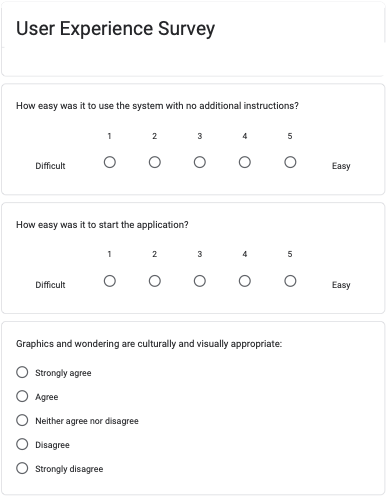
\includegraphics[width=1\textwidth]{VnV Plan/User Experience Survey1.png}
  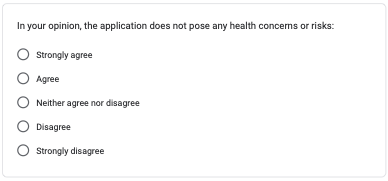
\includegraphics[width=1\textwidth]{VnV Plan/User Experience Survey2.png}
 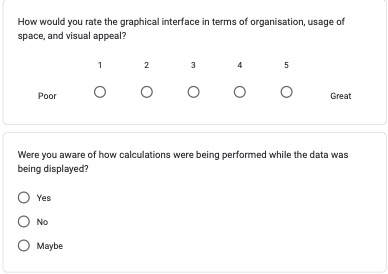
\includegraphics[width=1\textwidth]{VnV Plan/User Experience Survey3.jpg}

\end{document}